\documentclass[a4paper]{article}

% Links
\usepackage[pdftex, colorlinks, urlcolor=blue, linkcolor=black]{hyperref}
\usepackage{mathtools}
\usepackage[utf8]{inputenc}
\usepackage[spanish]{babel}
\usepackage[T1]{fontenc}
\usepackage{lmodern}
\usepackage{graphicx}
\usepackage{lastpage}
\usepackage{listings}
\usepackage{fancyhdr}
\usepackage{url}
\usepackage{color}
\usepackage{fullpage}
\usepackage{float}
\usepackage{booktabs}
\usepackage{mathtools}
\usepackage{subcaption}
\usepackage{blindtext}
\definecolor{lightgray}{rgb}{0.95,0.95,0.95}

\lstloadlanguages{Haskell}

\graphicspath{ {images/} }

\setlength{\footskip }{20pt}
\setlength{\headsep }{30pt}
\setlength{\headheight}{13pt}
\addtolength{\textheight}{-40pt}

\lstset{
  frame=none,
  xleftmargin=25pt,
  stepnumber=1,
  numbers=left,
  numbersep=5pt,
  numberstyle=\ttfamily\tiny\color[gray]{0.3},
  belowcaptionskip=\bigskipamount,
  captionpos=b,
  escapeinside={*'}{'*},
  language=haskell,
  tabsize=2,
  emphstyle={\bf},
  commentstyle=\it,
  stringstyle=\mdseries\rmfamily,
  showspaces=false,
  keywordstyle=\bfseries\rmfamily,
  columns=flexible,
  basicstyle=\small\sffamily,
  showstringspaces=false,
  morecomment=[l]\%,
  backgroundcolor=\color{lightgray},
}

\urlstyle{same}
% \title{Organización de Datos\\Diseño del Trabajo Práctico}
% \date{24 de Septiembre del 2015}
% \author{Tomás Arjovsky, Vsevolod Gavrilov, Nicolás Ledesma}

\begin{document}

\begin{titlepage}
  \centering
  \includegraphics[width=0.15\textwidth]{example-image-1x1}\par\vspace{1cm}
  {\scshape\LARGE{Universidad de Buenos Aires}} \\
  {\Large{Facultad de Ingenieria}\par}
  \vspace{1cm}
  {\scshape\Large Diseño del Trabajo Práctico \par}
  \vspace{1.5cm}
  {\huge\bfseries Clasificación de Crímenes en\\ San Fransisco\par}
  \vspace{2cm}
  {\Large\textsc{Organización de Datos}}
  \vfill
  {Tomás Arjovsky\\ Vsevolod Gavrilov\\ Nicolás Ledesma \par}

  \vfill

% Bottom of the page
  {\large \today\par}
\end{titlepage}

% \maketitle

\pagestyle{fancy}
\lhead{\slshape \leftmark}
\rhead{Página \thepage\  de  \pageref{LastPage}}
\chead{\scalebox{0.1}{asasasa}}
\lfoot{Universidad de \\ Buenos Aires}
\cfoot{Organización \\ De Datos}
\rfoot{Arjovsky, Gavrilov, Ledesma\\}
\renewcommand{\headrulewidth}{0.4pt}
\renewcommand{\footrulewidth}{0.4pt}

  \tableofcontents
  \clearpage

  \section{Introducción} % (fold)
\label{sec:introducci_n}

El trabajo práctico consiste en proponer una solución a la consigna de una competencia abierta en Kaggle, una plataforma de la comunidad de Data Science. La competencia consiste en la predicción de los crímenes ocurridos en San Fransisco a partir de los datos proporcionados. Estos datos se dividen en un \textit{set de entrenamiento}, un archivo csv, donde cada fila representa un crímen y cada columna proporciona información acerca de él, y un \textit{set de prueba}. Este último tiene el mismo formato, pero en las filas no se menciona de que crímen se está tratando. Queda a cargo de los participantes el deducir la probabilidad de la ocurrencia de cada \textit{clase} de crímen para cada fila del set de prueba.


Nosotros vamos a encarar el problema de la predicción de las clases de crímen utilizando varios algoritmos de \textit{machine learning}: \textbf{Regresión Logística}, \textbf{Red Neuronal} (y analizaremos otros algoritmos posibles). Dependiendo de la calidad de la solución de cada algoritmo, juntaremos los mejores \textit{modelos} para tener un resultado más preciso. Necesitaremos procesar y preparar los datos, extraer los diferentes atributos (o \textit{features}) del set de datos para que los algoritmos se entrenen de manera más eficiente. La solución final va a estar escrita en \textbf{C++}, pero realizaremos pruebas en lenguajes de más alto nivel (\textbf{Python} mayormente), aprovechando las herramientas de ML y procesamiento de datos existentes.

% section introducci_n (end)


  % \section{Acerca del equipo} % (fold)
\label{sec:acerca_de}

\subsection{Filosofía de trabajo} % (fold)
\label{sub:filosofia}

Nuestra filosofía para encarar esta competencia fue primeramente reunir toda la información y el conocimiento que creimos necesario para entender el problema. Para esbozar una solución y desarrollar un algoritmo de aprendizaje que consiga hacer una clasificación óptima de los crímenes de San Francisco decidimos primero entender el problema en sus distintas aristas. Esto implicó entre otras cosas:

\begin{itemize}
  \item Revisar los comentarios hechos hasta el momento en los foros de Kaggle. La competencia lleva ya varios meses de desarrollo, y es una buena forma de hacer un primer acercamiento aprender de los comentarios de los participantes que ya comenzaron a desarrollar su solución.
  \item Investigar acerca del dominio del problema planteado en la competencia. Las características geográficas de la ciudad de San Francisco, el grado de importancia de los features incluidos en el set de entrenamiento y el set de evaluación. Análisis y comprensión del significado de los features. Por ejemplo, entender qué tipo de eventos comprende la categoría de crimen ``Non criminal''. 
  \item Compartir los conocimientos previos de los integrantes del equipo en el campo de Data Science, más específicamente en el área de machine learning. Complementar estos conocimientos previos con nuevas investigaciones que nos permitan aprender el funcionamiento de los algoritmos de machine learning existentes, y aún más importante, la idoneidad de los mismos para abordar este problema.
\end{itemize}

\subsection{Plan de trabajo} % (fold)
\label{sub:plan}

Desde la conformación del equipo nos dedicamos primeramente a hacer investigaciones con la extensa información que hay en internet, ya sea para aprender los algoritmos, como el dominio del problema y la matemática involucrada.

A continuación, una vez aprendidas las nociones básicas de varios algoritmos y soluciones posibles, pasamos a investigar sobre posibles librerías que nos faciliten el tratamiento de los features de los sets de entrenamiento y evaluación, así como la implementación de algunos de los algoritmos investigados. Así fue como encontramos comodidad en el entorno que ofrece python para rápidamente procesar los datos de entrada y simular, a través de librerías como el Sci-kit, los algoritmos que más nos llamaron la atención y nos parecieron útiles para desarrollar una solución.

Simultáneamente evaluamos y propusimos diversas formas de generar nuevos features a partir de los que aporta el set de entrenamiento. Consideramos que la forma de representar la información otorgada por la competencia, y de alimentar los algoritmos es clave para lograr un aprendizaje más eficiente en ellos.

Finalmente comenzamos a pensar en la implementación de los algoritmos que más nos gustaron en C++, y las librerías que consideramos útiles para facilitarlo. De aquí en adelante resta comenzar a desarrollar la implementación, y dejar abierta la posibilidad de combinar soluciones para obtener mejores resultados.

  % Los algoritmos consumen numeritos y nosotros tenemos palabritas...... Como convertir datos, que variables usar, que features pensamos, graficos, conclusiones sobre los graficos, etc. Posibles datos externos.
  % Los X e Y que estan afuera
  
\section{Tratamiento de datos} % (fold)
\label{sec:tratamiento_de_datos}

\begin{table}[!htbp]
\centering
\resizebox{\textwidth}{!}{

\begin{tabular}{lllllllrr}
\toprule
               Dates &        Category &     Descript &  DayOfWeek & PdDistrict &      Resolution &                  Address &           X &          Y \\
\midrule
 2008-04-15 18:30:00 &   DRUG/NARCOTIC &  POSSESSI... &    Tuesday &       PARK &  JUVENILE CITED &  700 Block of STANYAN ST & -122.453513 &  37.768697 \\
 2011-08-25 18:33:00 &        WARRANTS &  WARRANT ... &   Thursday &   SOUTHERN &  ARREST, BOOKED &   900 Block of MARKET ST & -122.408421 &  37.783570 \\
 2007-09-09 02:32:00 &     DRUNKENNESS &  UNDER IN... &     Sunday &   SOUTHERN &  ARREST, BOOKED &  1400 Block of FOLSOM ST & -122.413772 &  37.772142 \\
 2012-09-08 23:59:00 &   LARCENY/THEFT &  GRAND TH... &   Saturday &  INGLESIDE &            NONE &   100 Block of EMMETT CT & -122.416079 &  37.747295 \\
 2004-03-17 16:00:00 &   LARCENY/THEFT &  GRAND TH... &  Wednesday &   SOUTHERN &            NONE &   CLEMENTINA ST / 5TH ST & -122.403924 &  37.780699 \\
 2014-06-01 00:20:00 &        BURGLARY &  BURGLARY... &     Sunday &   NORTHERN &            NONE &  1300 Block of SUTTER ST & -122.422586 &  37.787387 \\
 2008-07-10 18:15:00 &  OTHER OFFENSES &  DRIVERS ... &   Thursday &   SOUTHERN &   ARREST, CITED &     HARRISON ST / 1ST ST & -122.392941 &  37.786068 \\
 2003-05-13 12:00:00 &   LARCENY/THEFT &  PETTY TH... &    Tuesday &   NORTHERN &            NONE &  0 Block of CERVANTES BL & -122.438303 &  37.803634 \\
 2013-04-07 19:00:00 &    NON-CRIMINAL &  FOUND PR... &     Sunday &   SOUTHERN &            NONE &     300 Block of 10TH ST & -122.412410 &  37.772404 \\
 2014-06-25 22:15:00 &   LARCENY/THEFT &  GRAND TH... &  Wednesday &   SOUTHERN &            NONE &      FOLSOM ST / 10TH ST & -122.412827 &  37.772812 \\
\bottomrule
\end{tabular}


}
\caption{Algunos datos aleatorios del set de entrenamiento}
\end{table}

\subsection{Explorando el set de datos} % (fold)
\label{sub:explorando_el_set_de_datos}

Los sets de datos son extensos. Para darnos una idea de como están compuestos podemos tomar una muestra, y analizarla. Cada fila del set representa un crimen. Las filas vienen con una fecha completa, el distrito donde pasó el crimen, el día de semana, la dirección, la latitud y la longitud exactas. El set de entrenamiento también viene con el tipo de cada crimen (los que justamente necesitamos deducir sobre el set de prueba), y con una descripción y resolución de cada crimen. Estos últimos dos no nos interesan, ya que no aparecen en el set de prueba y, por ende, no podremos tomar ninguna decisión en base a ellos.

Pero para entender mejor el set de datos, lo graficaremos. Teniendo, por ejemplo, el gráfico de categorías~\ref{fig:categories} ya podemos hacer deducciones sobre nuestro set de entrenamiento. Es muy visible que los crímenes no están uniformemente distribuidos, por ende lo más probable es que en la deducción casi siempre vamos a tender a darle más probabilidad a \textit{LARENCY/THEFT} o \textit{OTHER OFFENSES}.

\begin{figure}[H]
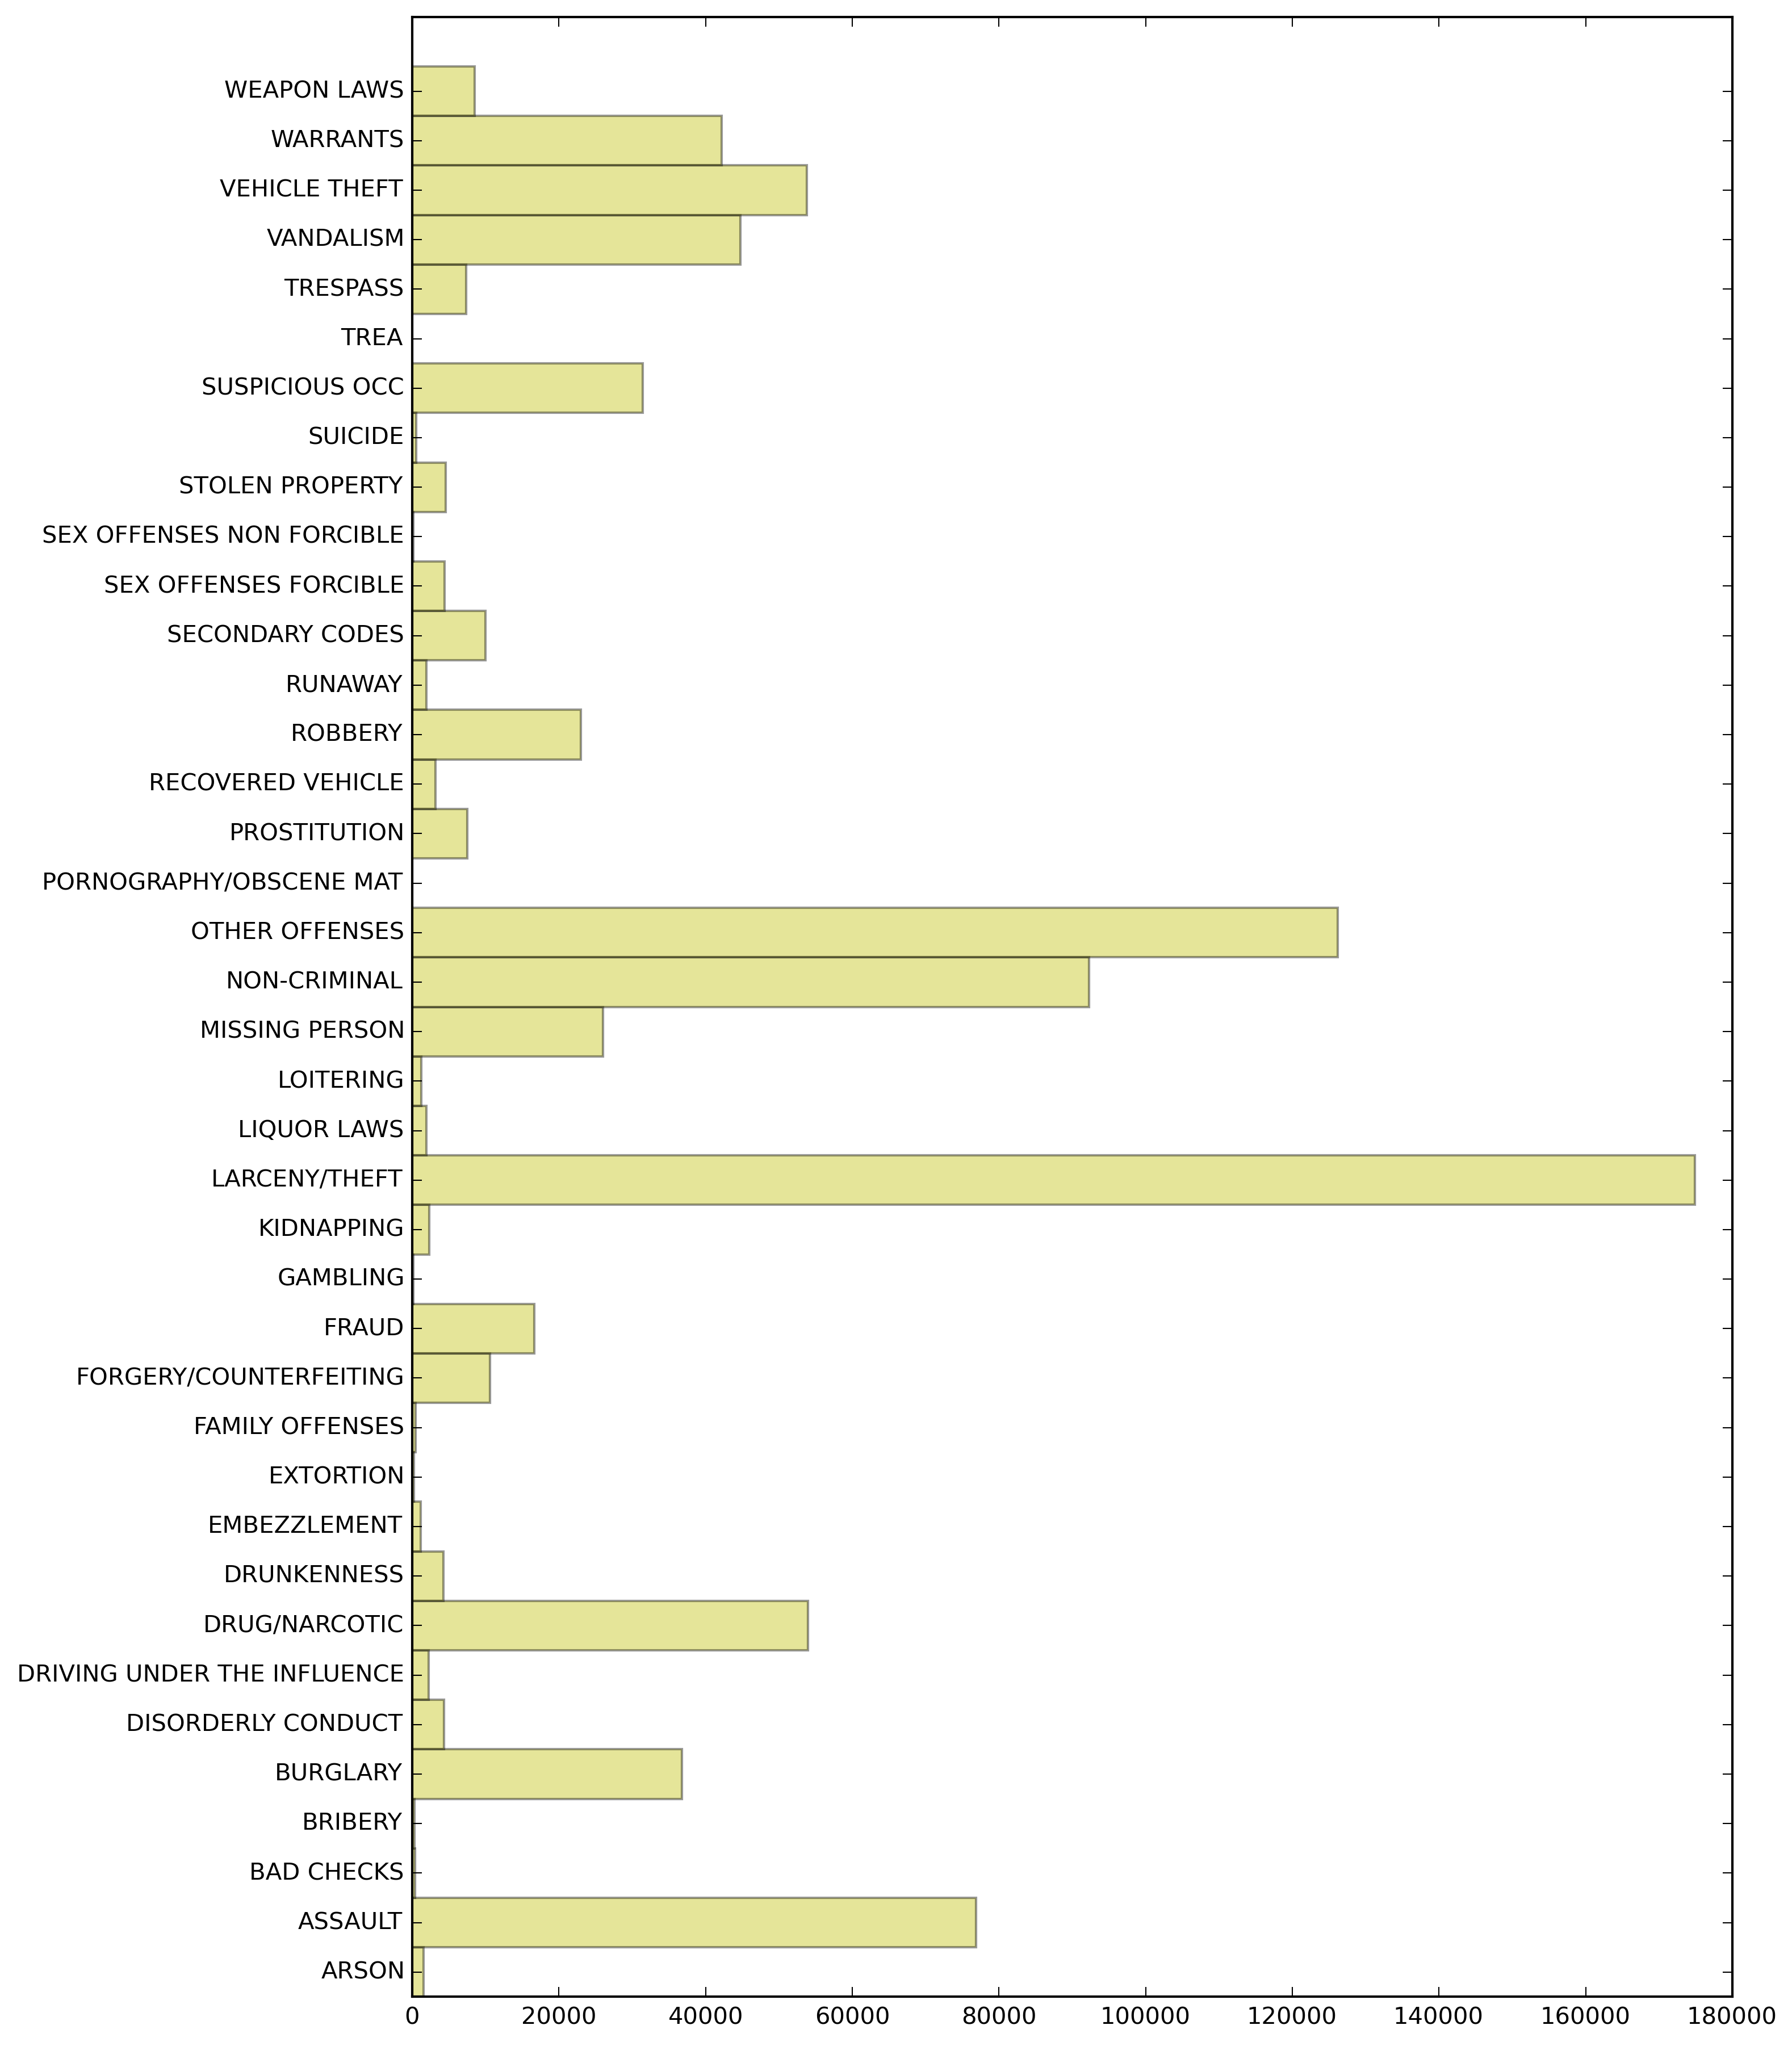
\includegraphics[width=130mm]{categories}
\caption{Cantidad de crímenes de cada tipo.}
\label{fig:categories}
\end{figure}

% subsection explorando_el_set_de_datos (end)

\subsection{Deduciendo features} % (fold)
\label{sub:deduciendo_features}

Como parte de preprocesamiento, necesitaremos deducir cuáles son los datos importantes para nosotros, es decir cuáles son los datos que van a ayudar a que nuestro algoritmo aprenda más eficientemente y prediga mejor. Esos datos se pueden encontrar directamente en el set de datos tal como está o pueden necesitar algún procesamiento previo. Algunos inclusive pueden ser combinación de varios datos de una fila.

Los únicos datos discretos, que sirven directamente son el distrito y el día de semana. La fecha tal como viene no tiene valor: cada crimen tiene una fecha única y lo más probable es que en el set de prueba tampoco se repita. Necesitamos procesar esa fecha primero.

\begin{figure}[H]
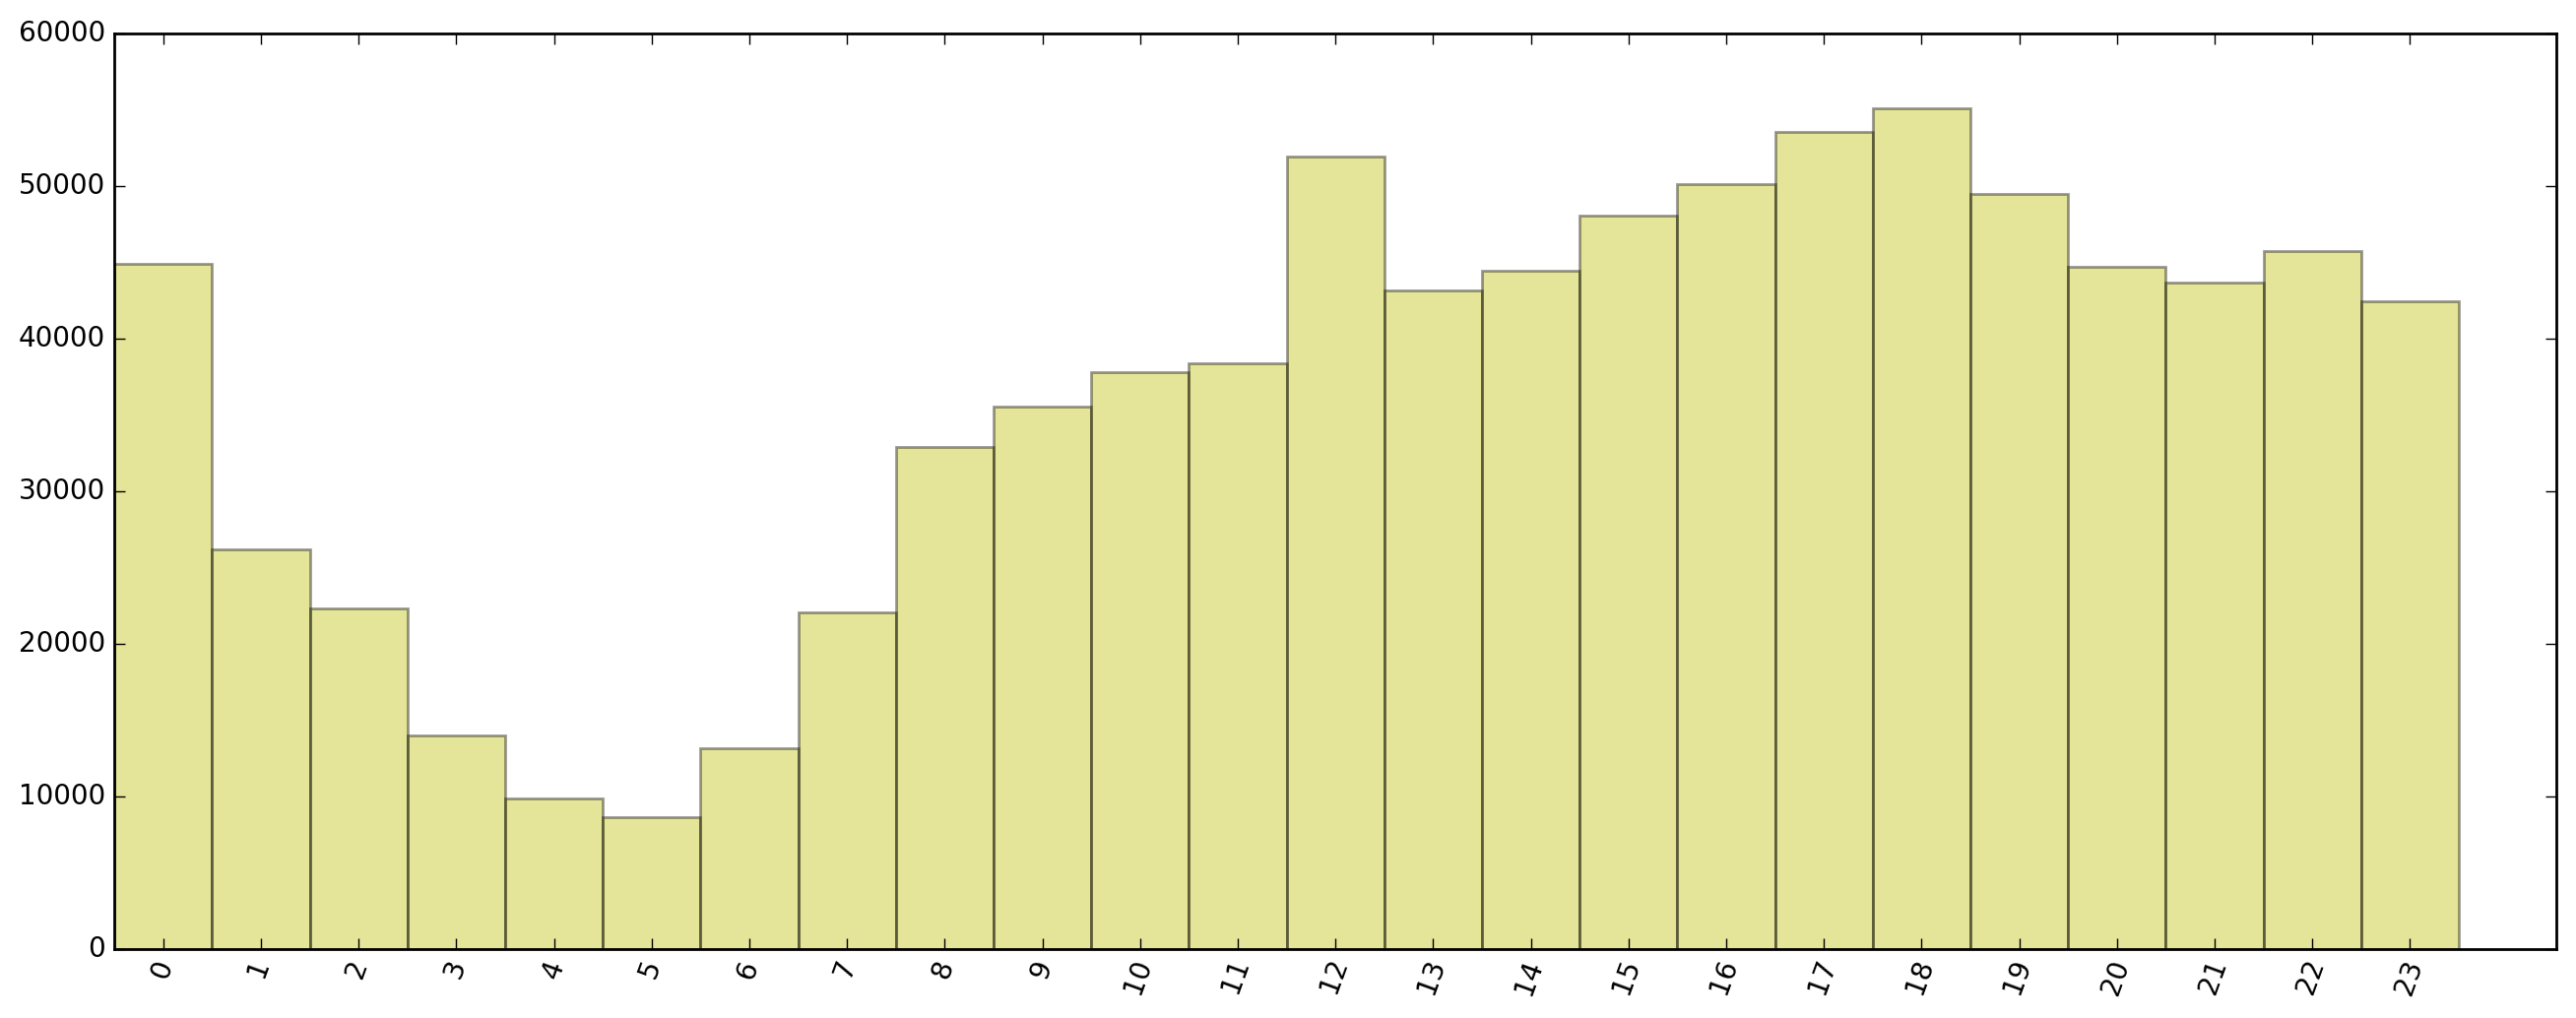
\includegraphics[width=160mm]{hours}
\caption{Cantidad de crímenes por hora.}
\label{fig:hours}
\end{figure}

Fecha es un dato muy útil, algunos features resultantes del procesamiento de ella que vienen inmediatamente a la mente son: la hora, el mes, el año. Pero podemos sacar otros features no menores, por ejemplo deducir si era verano o invierno, si era de día o de noche (inclusive variar el rango de día y de noche según estación, siendo que en invierno oscurece más temprano). Sí observamos el gráfico~\ref{fig:hours}, podemos detectar que entre la una y las siete la cantidad de crímenes baja notablemente y, por lo contrario, hay dos picos a las 12 y a las 18. Todos esos datos se pueden convertir en features para nuestro algoritmo. También podemos sacar el dato sobre el día de semana de la fecha - de esta forma la columna con el día de semana en los sets es, en realidad, redundante. Si podemos conseguir datos externos, podríamos que fechas fueron feriado.

La dirección a priori no es un dato tan fuerte como la fecha, y también necesita procesamiento. Podríamos sacar nombres de calles o abusarnos de la notación y deducir que crímenes ocurrieron en las esquinas (las dirección de las esquinas están denotadas como ``Calle 1 / Calle 2''.

La longitud y la latitud es a simple vista un dato muy importante y a la vez difícil de procesar. Eso pasa por el hecho de que por separado claramente no tienen sentido. Vamos a tener que encontrar una forma de convertirlos en algo útil para nuestros algoritmos. Una manera podría ser encontrar alguna función que devuelva un número muy parecido para X e Y cercanos. Otra sería dividir las longitudes y latitudes en zonas, y ver en que zona se encuentra la fila. Este enfoque puede conducir a errores ya que para ser preciso va a necesitar más zonas. Algo útil podría resultar una búsqueda de datos externos con latitudes y longitudes de lugares particulares de San Francisco, como pueden ser las estaciones de policía (distancia a ellos podría ser un feature interesante), o determinar si el crimen pasó en un parque.

\begin{figure}[H]
\centering
\begin{subfigure}{.5\textwidth}
  \centering
  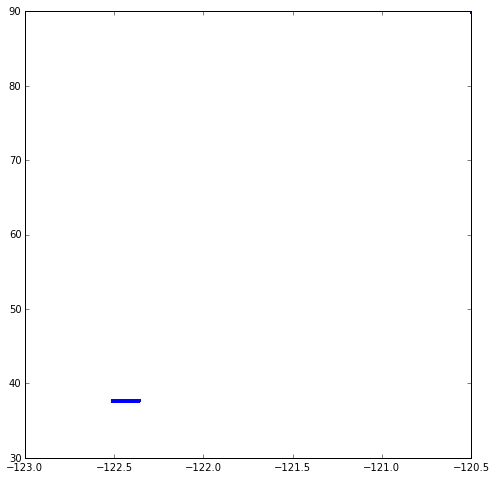
\includegraphics[width=.8\linewidth]{xy1}
  \caption{Set de entrenamiento}
  \label{fig:xy1}
\end{subfigure}%
\begin{subfigure}{.5\textwidth}
  \centering
  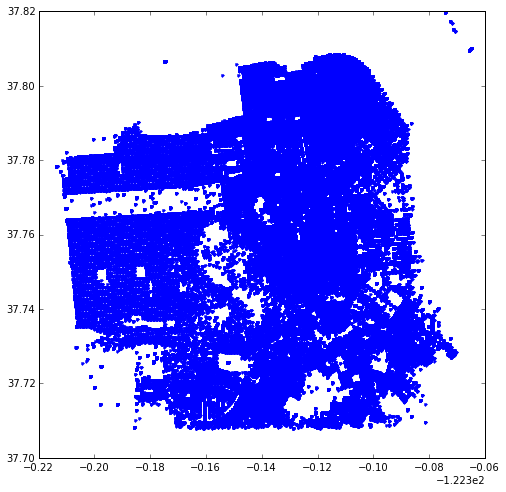
\includegraphics[width=.8\linewidth]{xy2}
  \caption{Sin datos incorrectos}
  \label{fig:xy2}
\end{subfigure}
\caption{Gráficos de latitudes y longitudes de los crímenes}
\label{fig:xy}
\end{figure}

Si graficamos la latitud en función de la longitud, lo primero que vamos a obtener es algo parecido al gráfico de~\ref{fig:xy2}: nos encontramos con que algunas de las filas tienen datos incorrectos. Hay 67 crímenes con latitudes y longitudes incorrectas. Si bien podríamos descartarlos - su impacto es minucioso frente al set entero, pero es posible, por ejemplo determinar su X e Y correcto a partir de los crímenes que pasaron en las mismas direcciones. Y para los que queden sin clasificar - podríamos ubicarlos en lugares aleatorios de San Francisco.

% subsection deduciendo_features (end)


\subsection{Transformando datos} % (fold)
\label{sub:transformando_datos}

El set de datos proporcionado en su estado inicial no sirve para aplicarle los algoritmos típicos de machine learning: un algoritmo matemático no tiene una forma práctica de interpretar los datos que contiene. Los datos que mejor puede interpretar son números. Entonces está entre nuestras necesidades el convertir los sets de datos heterogéneos en matrices numéricas.

Todos los features necesitan ser escalados a un rango de números (puede ser entre 0 y 1, o entre -1 y 1). De esta manera el algoritmo tiene menor chance de equivocarse dándole mayor peso a features con mayor valor numérico (como puede ser el año con respecto al mes).

¿Pero como hacemos para representar numéricamente si un crimen pertenece a un distrito? Una de las solución es utilizar codificación \textit{one-hot} (o variables \textit{dummy}). Este método consiste en, en vez de representar alguna variable categórica, como puede ser el distrito, con un solo feature, representarlo con un feature por cada categoría existente, marcando si es o no es de esa categoría (con un 1 o un 0). De esa manera a partir de la columna de Distrito tendríamos 10 features diferentes, donde cada fila tendría un 1 en uno de ellos - y 0 en el resto. Lo mismo es posible hacerlo con los días de semana, meses, años, zonas de latitudes y longitudes, y hasta calles - pero es necesario hacer un análisis previo y decidir si tiene sentido o no.

% subsection transformando_datos (end)

% section tratamiento_de_datos (end)


  % Algoritmos a usar (algoritmos probados, submissions, etc.) Explayarse sobre el algoritmo, consta de tales partes, y eso.
  
\section{Algoritmos de predicción} % (fold)
\label{sec:algoritmos_de_prediccion}

\subsection{Regresión Logística} % (fold)
\label{sub:regresion_logistica}

La regresión logística a pesar de su nombre es un algoritmo de clasificación, el cual puede implementarse para realizar una clasificación binaria, o una clasificación de múltiples valores posibles.

El modelo de la regresión logística es análogo al de la regresión lineal, dado que tal como la misma, parte de una función hipótesis que se le aplica a los datos de entrada.
\begin{equation}
h_{\theta}(x)= \theta^T \cdot x
\end{equation}
\begin{small}
Esta es la representación vectorial de la función hipótesis de la regresión lineal. Donde $X$ es el vector traspuesto de datos $x_{i}$, y $\Theta^T$ es el vector de pesos $\theta_{j}$.
\end{small} \newline

En el caso de la regresión lineal, el valor de retorno de la función hipótesis puede variar mucho dependiendo del vector de datos de entrada $X$ y el vector de pesos $\Theta$. En este aspecto la regresión logística se diferencia de la regresión lineal.

\subsubsection{Función sigmoidal.}
En el caso particular de la regresión logística, la función hipótesis se construye de la siguiente manera:
\begin{equation}
h_{\theta}(x)= \frac{1}{1+e^{- \theta^T\cdot x }}
\end{equation}

Similarmente, la hipótesis de la regresión logística utiliza el vector de datos de entrada $X$ y el de pesos $\Theta$, y su función retorna un valor escalar. Sin embargo, esta nueva función otorga una ventaja al retornar un número escalar real comprendido entre 1 y 0. Este tipo de función se llama función sigmoidal, y el valor escalar comprendido entre 1 y 0 se puede interpretar como una probabilidad.
\begin{figure}[H]
\centering
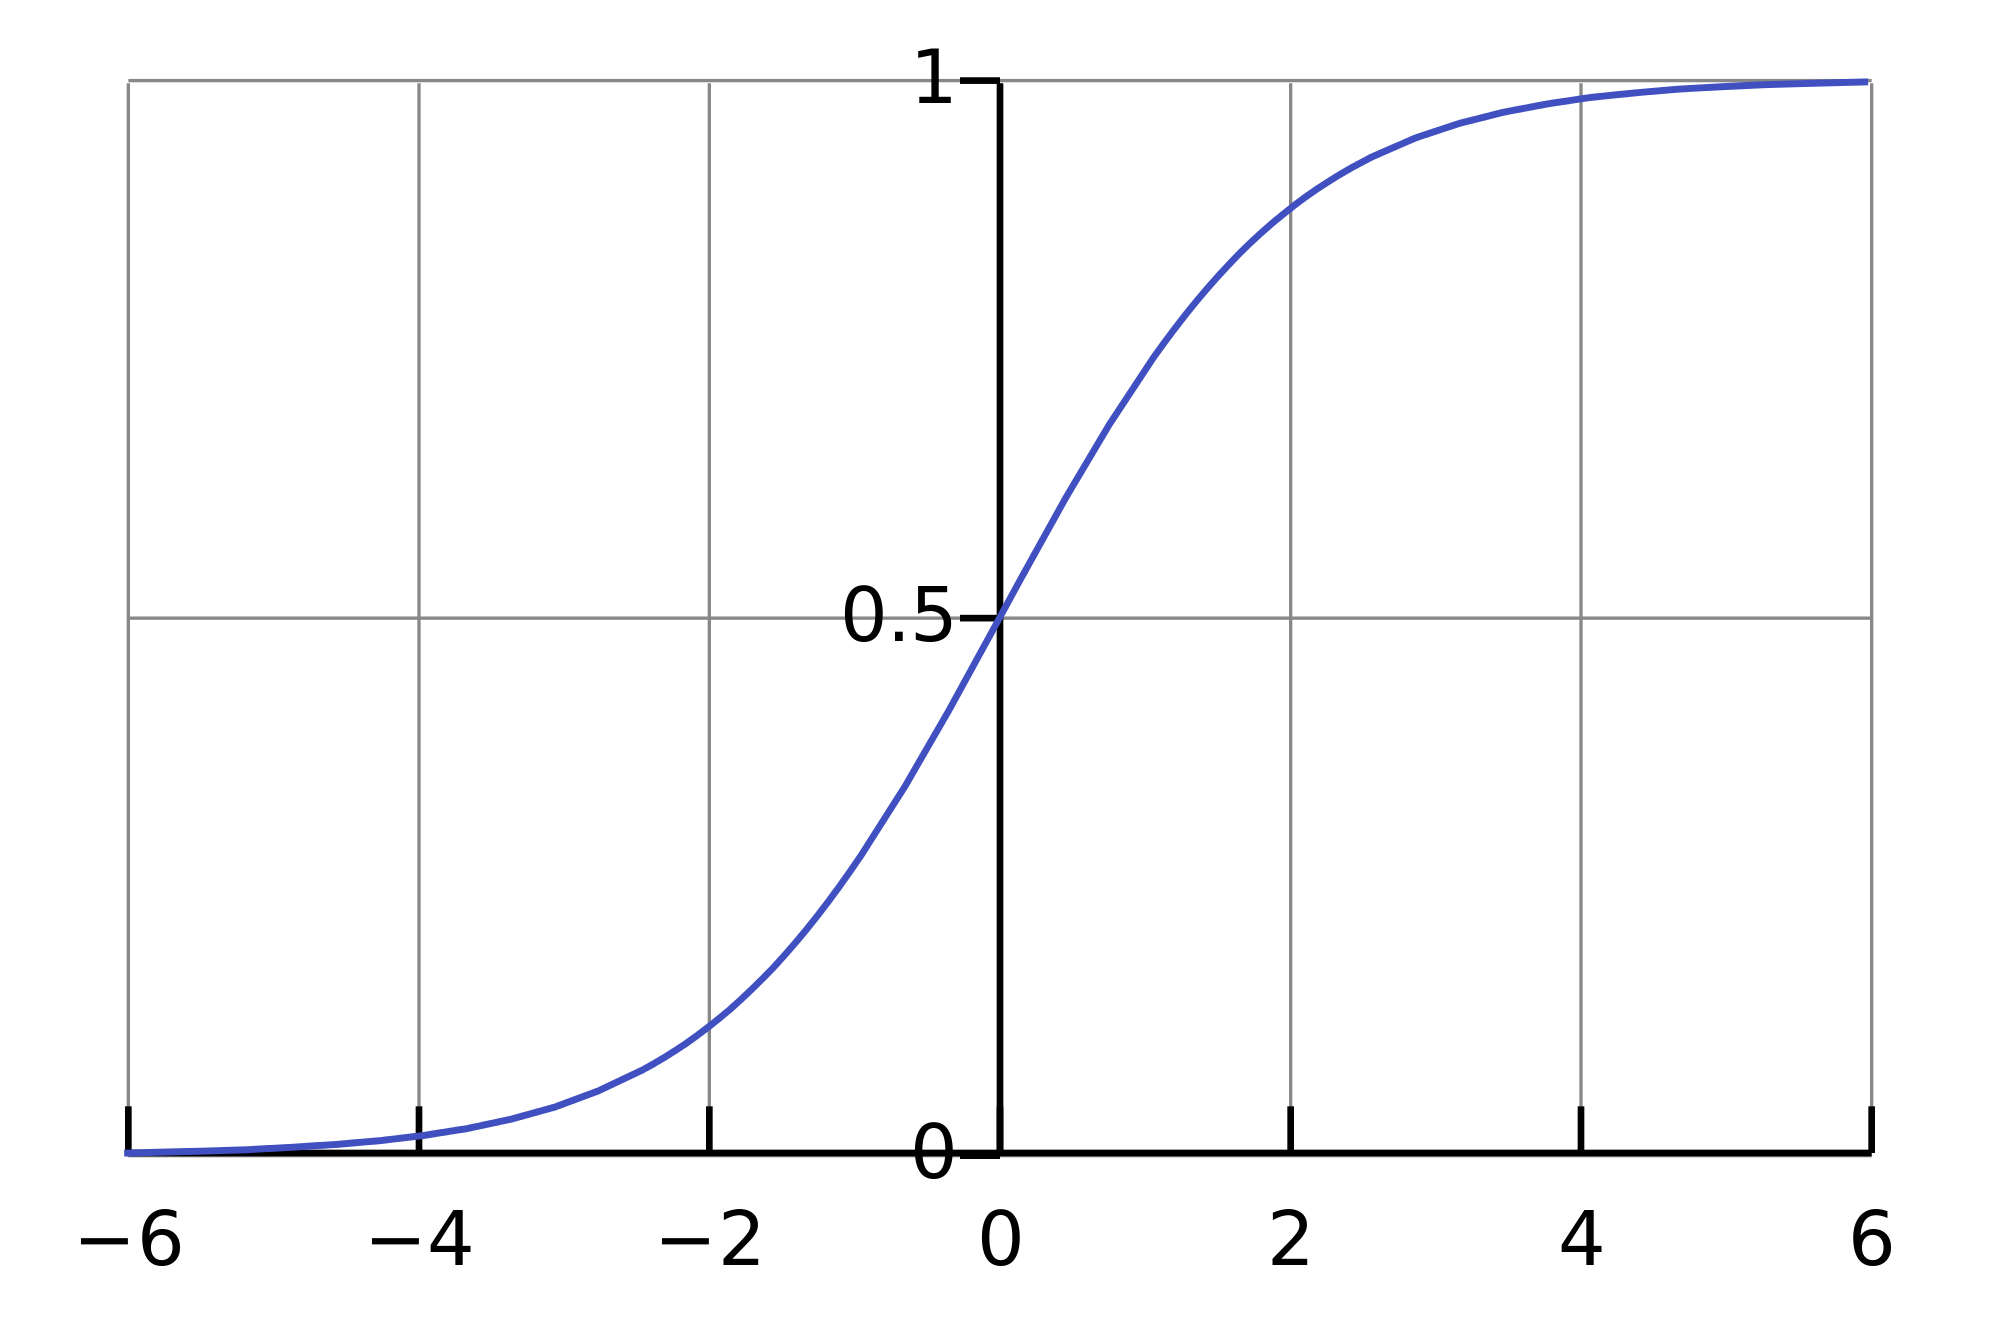
\includegraphics[width=80mm]{logisticCurve}
\caption{Gráfica de una función sigmoidal.}
\label{fig:logisticCurve}
\end{figure}

\subsubsection{Uno contra todos.}
Sin embargo, hasta el momento el algoritmo parece ser sólo diseñado para resolver problemas de clasificación binaria. Para utilizar este algoritmo de forma pueda abordar un problema de salida multiclase, debe aplicarse algún esquema de clasificación que aproveche las salidas binarias (o de probabilidad entre 0 y 1) de la función sigmoidal. Para eso se utiliza el esquema \textit{ovr (One-vs-rest)}. One-vs-rest no aplica otra cosa que el criterio de \textit{dividir y conquistar}. Por cada clase se resuelve el problema en forma binaria, donde el caso positivo (1) corresponde a la clase misma, y el caso negativo corresponde a cualquier otra clase. A continuación puede verse una representación gráfica de esta estrategia:

\begin{figure}[H]
\centering
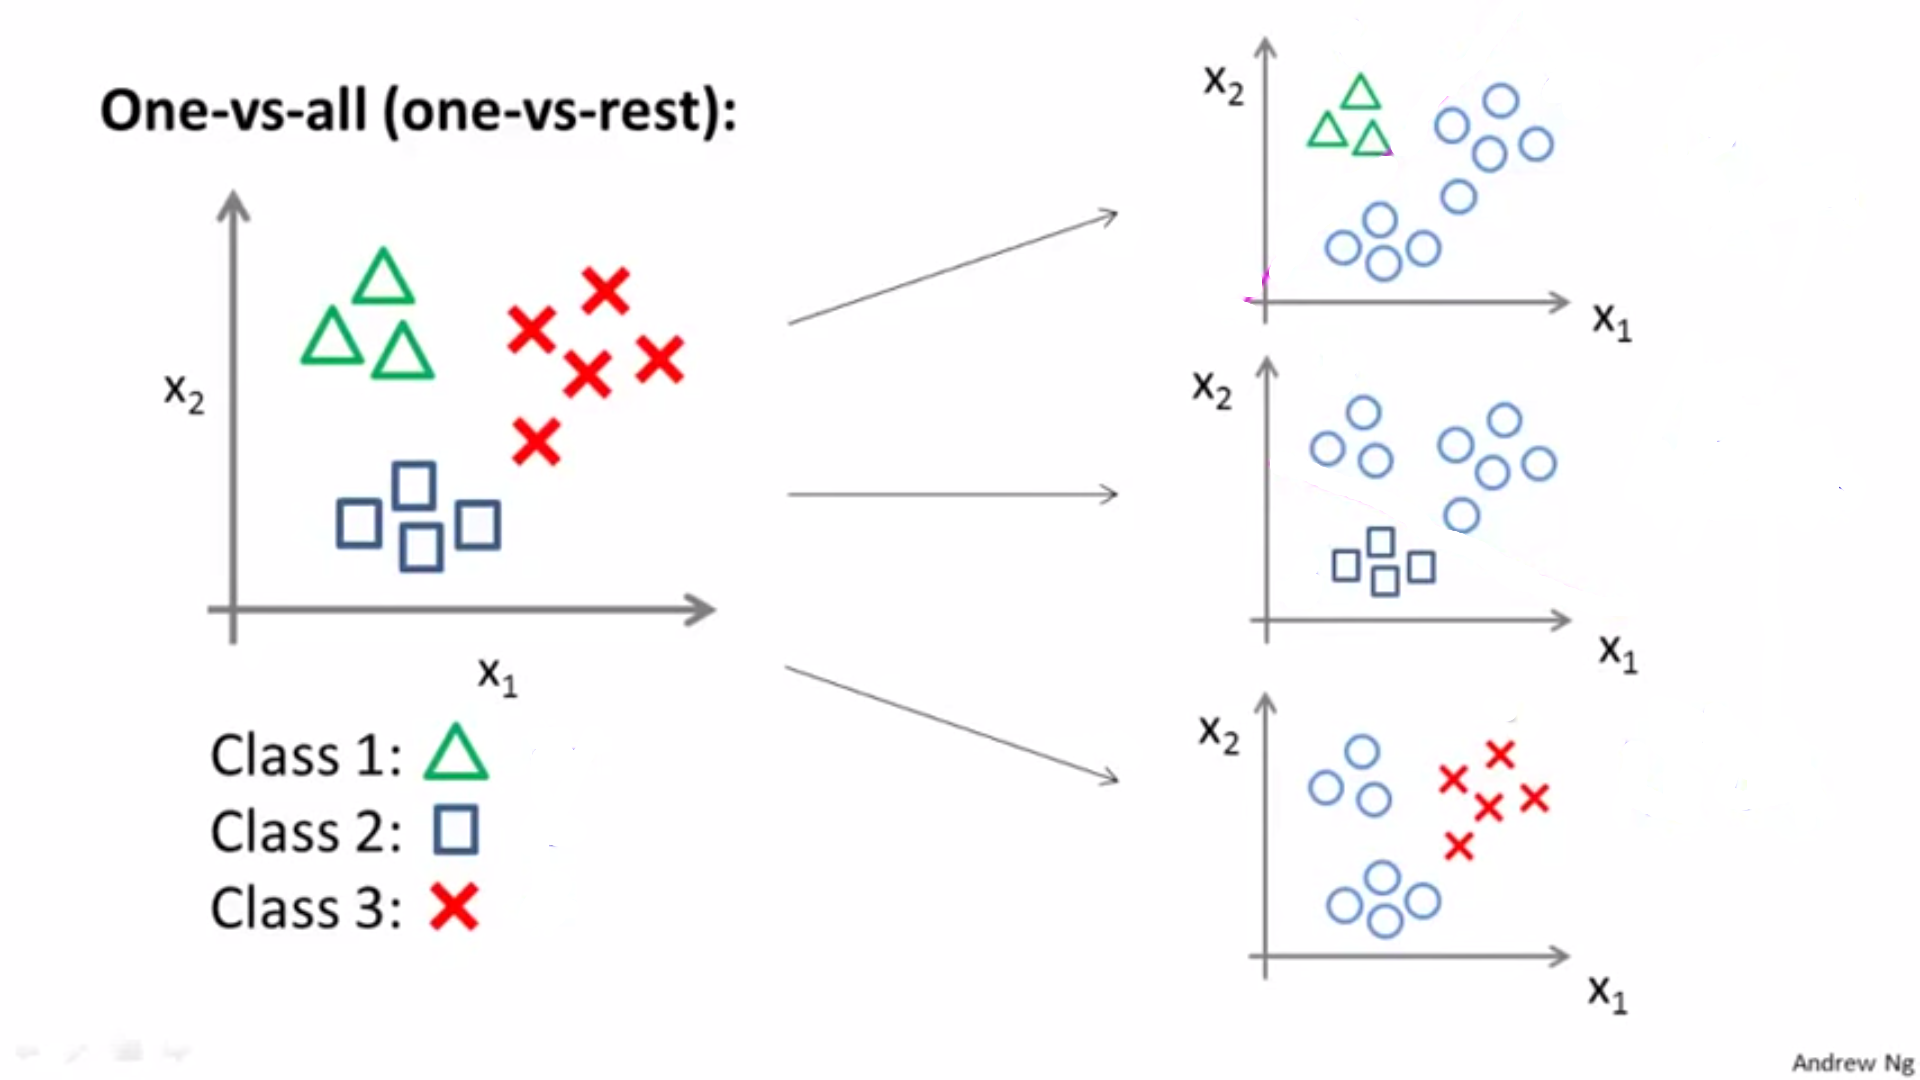
\includegraphics[width=80mm]{oneVsRest}
\caption{Representación gráfica one-vs-rest. \cite{AndrewNgMulticlass}}
\label{fig:oneVsRest}
\end{figure}

\subsubsection{Estimación y Función de Costo.}
De esta manera se cuenta con una serie de funciones $h_{\theta}^k(x)$ donde $k$ es el número de la clase que representa la función. A través del valor de retorno de todas estas funciones se obtiene entonces la probabilidad de cada clase distinta para cada caso del set de valores de entrada.

Este conjunto de probabilidades obtenido, es una estimación, y esa estimación debe aproximarse al valor deseado. En este trabajo disponemos de un set de entrenamiento asociado a las clasificaciones correctas. El objetivo de la regresión logística es esbozar una función de costo dados los pesos $\theta_{j}$ . De esta manera, optimizando (o minimizando) la función costo se pueden corregir los pesos $\theta_{j}$, de forma que las estimaciones posteriores se asemejen cada vez más a los valores deseados o ``correctos''.

A continuación se muestra un ejemplo ilustrativo de una definición de función de costo:

\begin{equation}
J(h_{\theta }(x),y) = \begin{cases}
- \log h_{\theta}(x) & \textit{si $y \equiv 1$} \\
- \log (1- h_{\theta}(x)) & \textit{si $y \equiv 0$}
\end{cases}
\end{equation}

La conveniencia de esta función de costo es que:

\begin{itemize}
  \item Cuando el valor esperado es $1$, y la estimación se aproxima a $0$, el costo tiende a $\infty$.
  \item Cuando el valor esperado es $1$, y la estimación se aproxima a $1$, el costo tiende a $0$.
  \item Cuando el valor esperado es $0$, y la estimación se aproxima a $1$, el costo tiende a $\infty$.
  \item Cuando el valor esperado es $0$, y la estimación se aproxima a $0$, el costo tiende a $0$.
\end{itemize}

Esto ocurre gracias a que las funciones logarítmicas de cada caso se comportan como describen las siguientes gráficas:

\begin{figure}[H]
\centering
\begin{subfigure}{.5\textwidth}
  \centering
  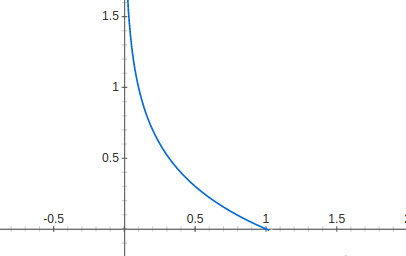
\includegraphics[width=.8\linewidth]{minusLogX}
  \caption{$y = - \log (x)$}
  \label{fig:minusLogX}
\end{subfigure}%
\begin{subfigure}{.34\textwidth}
  \centering
  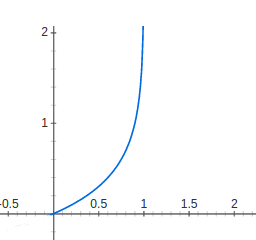
\includegraphics[width=.8\linewidth]{minusLog1minusX}
  \caption{$y = - \log (1-x)$}
  \label{fig:minusLog1minusX}
\end{subfigure}
\caption{Gráficas}
\label{fig:minusLog}
\end{figure}

Análogamente, se pueden definir funciones de costo de forma contínua, obteniendo comportamientos similares. En el caso particular de la clase LogisticRegression implementada en el paquete de python \textit{sklearn}, una función de costo utilizada es la siguiente:

\begin{equation}
J(\theta,c)= \theta^T \cdot \theta + C \sum_{i=1}^n \log (e^{-y_{i} \cdot (X_{i}^T \theta + c)})
\end{equation}
Donde:

\begin{itemize}
  \item $X_{i}$ es el vector de parámetros de entrada del i-ésimo caso de un set de entrenamiento.
  \item $y_{i}$ es el valor correcto conocido del i-ésimo caso de un set de entrenamiento.
  \item $c$ es una constante de ajuste, al igual que los pesos comprendidos en el vector $\theta$.
  \item $\theta^T \cdot \theta$ y $C$ son complementos de la función de costo pensados para regularizarla, suavizando su comportamiento con el fin de evitar cometer \textit{overfitting}.
\end{itemize}

\subsubsection{Optimización: descenso por el gradiente.}
Por último, queda detallar el método de optimización utilizado por la regresión logística. Los métodos de optimización de la función de costo pueden ser derivativos o no derivativos.

El método derivativo clásico es el descenso por el gradiente. El descenso por el gradiente consiste en calcular el gradiente de la función costo. De esta forma se obtiene la dirección y sentido de máximo crecimiento de la función. Con el fin de minimizarla, lo que se hace es, a través de un escalar que se denomina \textit{paso} de la optimización, se van variando los valores de $\theta_{i}$ en la misma dirección y sentido opuesto que el gradiente, de forma de apuntar hacia la minimización de la función de costo. Esto se realiza iterativamente, recalculando el gradiente de la función costo con los parámetros $\theta_{i}$ actualizados.

Sin embargo, las librería \textit{sklearn} utiliza en el modo \textit{liblinear} un método no derivativo denominado \textit{descenso coordenado} \cite{sklearnLinearModel}. El descenso coordenado consiste en partir la optimización en optimizaciones más simples, de una variable. Esto lo hace minimizando la función de costo por una coordenada o variable a la vez. Itera por cada variable y calcula la dirección de descenso de la función modificando el valor de esa sola variable.

A continuación se muestra una gráfica que ilustra este método de optimización:

\begin{figure}[H]
\centering
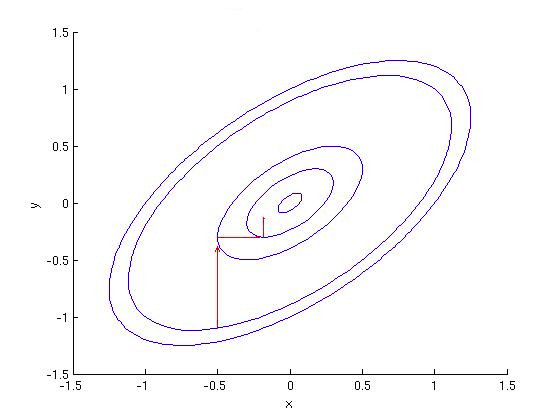
\includegraphics[width=80mm]{coordinateDescent}
\caption{Descenso coordenado. Las elipses concéntricas son curvas de nivel, donde el centro de las elipses se encuentra un mínimo local. \cite{wikipediaCoordinateDescent}}
\label{fig:coordinateDescent}
\end{figure}

En su forma vectorial, el descenso por el gradiente podría verse con la siguiente fórmula de actualización:
\begin{equation} \label{eq:gdesc}
\theta := \theta - \alpha \nabla J(\theta)
\end{equation}

\subsubsection{Feature Scaling}
Una mejora muy grande que se le puede hacer al descenso por el gradiente es la normalización o escalado de las variables de entrada (features). El problema que ataca es la diferencia entre los rangos de valores posibles de las features.

Por ejemplo, una variable puede ser la cantidad de cuartos que tiene una casa y otro la cantidad de metros cuadrados que tiene. Mientras uno se mueve entre 1 y 10 aproximadamente, el otro seguro será 10 veces más grande. Otros más comunes son, por ejemplo, la calificación del 1 al 5 de una película contra la cantidad de vistas que tiene, que pueden ser millones. Este desequilibrio produce, en gráficos como la figura \ref{fig:coordinateDescent}, que se haga cada vez más ovalado, y por lo tanto el paso $\alpha$ que tiene que dar en cada iteración para que no haya divergencia tiene que ser menor. Esto hace que sea más difícil de debuggear y que la convergencia, debido al paso más chico, sea mucho más lenta.

El feature scaling consiste en pasar todas las variables a intervalos aproximadamente entre 0 y 1 y luego entrenar $\theta$ sobre esas nuevas features normalizadas. El scaling se hace de la siguiente manera:

\begin{equation}
x_i := \frac{x_i - \mu_{x_i}}{\sigma_{x_i}}
\end{equation}

Al quitarle el valor medio y dividir por la desviación estandar, todas las variables quedan en rangos similares y el descenso por el gradiente puede hacerse de forma más segura y rápida.

Para poner un ejemplo concreto, probando un ajuste de parábolas por regresión lineal, sin escalamiento de variables requería un $\alpha$ más pequeño que 0.0001 para converger y por lo tanto miles de iteraciones. Por otro lado, escalando las variables, había convergencia con un paso de 1.0 y en algunas decenas de iteraciones ya se conseguían errores menores a $10^{-15}$.

\subsubsection{Regularización}
Como fue mencionada antes, la regularización es una medida que se toma en contra del overfitting. El overfitting, o sobreajuste, es un problema que consiste en que el algoritmo predictor quede muy bien entrenado para el predecir dentro del set de entrenamiento, pero no tenga capacidad de generalizar. Esto suele ocurrir cuando se modela un problema con una complejidad mayor a la que le corresponde, o cuando faltan ejemplos para la cantidad de features que se proponen.

A veces quitar features no es una opción. Sin embargo, si se puede penalizar darle mucha importancia a todos los features a la vez. Esta penalización se hace a través del costo y se llama regularización:

\begin{equation}
J(\theta) = -\frac{1}{m}\sum_{i = 1}^{m}\left[y^{(i)}(log(h_\theta(x^{(i)}))) + (1-y^{(i)})log(1-h_\theta(x^{(i)}))\right] + \frac{1}{m}\sum_{j = 1}^{n}\theta_j^2
\end{equation}
Y en forma vectorial:
\begin{equation}
J(\theta) = \frac{1}{m}\left[ -y^Tlog(h_\theta(x)) - (1-y)^Tlog(1-h_\theta(x)) + \theta^T\theta\right]
\end{equation}

De todos modos hay que tener en cuenta que no se regulariza el parámetro del término independiente, con lo cual en el término de la derecha ($\theta^t\theta$) deben extraerse primero los $\theta_0$.

\subsubsection{Stochastic Gradient Descent}
Para conjuntos de datos muy grandes, tales como el que se nos presenta de crímenes en San Francisco, puede ser muy costoso sumar sobre todos los 800.000 ejemplos antes de avanzar un paso. El descenso por el gradiente estocástico, mezcla aleatoriamente los ejemplos y luego va iterando sobre aquellos, en cada paso bajando por la contribución que tiene cada uno al gradiente.

El descenso por el gradiente clásico (en tanda), según lo expuesto en la ecuación \ref{eq:gdesc}, puede expresarse componente a componente:
\begin{equation}
\theta_j := \theta_j - \alpha\frac{1}{m}\sum_{i = 1}^{m}(h_\theta(x^{(i)}) - y^{(i)})x_j^{(i)}
\end{equation}
Pero podemos observar que las componentes de la sumatoria son la parte que cada ejemplo contribuye al gradiente. Tomando este concepto, en lugar de sumar todos los valores antes de avanzar, el descenso por el gradiente estocástico baja un poco por cada ejemplo que recorre, a través de la contribución que este otorga al gradiente \cite{andrewStock}.

\begin{equation}
\theta_j := \theta_j - \alpha(h_\theta(x^{(i)}-y^{(i)}))x_j^{(i)}
\end{equation}
Esto último se hace para cada uno de los ejemplos y luego se vuelve a comenzar con el primero, hasta que el resultado sea el deseado.

Una variante de este método es una mezcla entre el descenso por el gradiente en tanda y estocástico, que agarra pequeñas tandas, de por ejemplo, 10 casos de entrenamiento cada una. Esto permite aprovechar las ventajas de vectorizar las cuentas que provee la versión en tanda y la ventaja de no tardar tanto tiempo hasta hacer un paso que provee la implementación estocástica.

Este algoritmo será útil también en las redes neuronales, que utilizan descenso por el gradiente.

\subsubsection{Entrega en Kaggle}
En particular, con una implementación rudimentaria en python utilizando solo el distrito y features basados en la fecha, sin ninguna de todas las mejoras aquí planteadas, se obtuvo un puntaje de 2.59489.

Aplicando este algoritmo sobre un subset de entrenamiento como prueba se obtenían predicciones de precisión muy similar al set de entrenamiento, que rondaba el 22\% de acertadas.
\subsection{Redes Neuronales}



  % los4JinetesDeLaEntropia
  
\subsection{Otros Algoritmos} % (fold)
\label{sub:otros_algoritmos}

\subsubsection{Random Forest} % (fold)
\label{ssub:random_forest}

Este algoritmo, conocido en castellano como ``Selvas Aleatorias'' es un algoritmo de ensamblado que combina varios algoritmos \textit{debiles} (por si solos no logran una clasificación eficiente) para construir un resultado mejor. Random Forest consta de varios arboles de predicción que se entrenan de forma independiente, cada uno con un subset de features de los datos de entrada - de esta manera se obtiene una colección de arboles no correlacionados. Para obtener la predicción final, los resultados de cada arbol se promedian. Para obtener resultados se le pueden variar la cantidad de arboles a usar, la cantidad de features por arbol (suele ser bastante más chica que la cantidad de features total, como la raiz cuadrada de ella, por ejemplo) y la profundidad de cada arbol.

El concepto es interesante, pero su aplicación con nuestro set falló en la práctica. Hemos hecho pruebas con las implementaciones de Random Forest de \textbf{scikit}. Dió excelentes resultados sobre el set de entrenamiento, primero entrenado, y luego con las predicciones sobre subsets de los datos de entrenamiento se obtiene un score mayor a 90\% y un \textit{logloss} de \~0.4. Pero se equivoca mucho sobre los datos que no conoce - al entrenarlo con un subset de entrenamiento y probarlo con otro subset, el score se vuelve muy bajo y el \textit{logloss} altisimo. La submisión a Kaggle nos resultó en un \textit{logloss} de 19.25726, usando como features el distrito, los días de semana, la hora, el mes y el año. Cabe destacar que solo lo hemos probado 1 vez, con 10 arboles y sin limitarle la profundidad a cada arbol - tendríamos que hacer pruebas variando esos parametros. Acá nos enfrentamos con otro problema - la implemetación de \textit{scikit} de RandomForest consume demasiada memoria RAM - dicho entrenamiento y posterior predicción usaron los 6GB de una notebook. Por otro lado, la aplicación fue muy rápida, tardando unos pocos minutos.

% subsubsection random_forest (end)

\subsection{Support Vector Machine} % (fold)
\label{sub:support_vector_machine}

El método conocido bajo este nombre es un modelo para aprendizaje supervisado. Este modelo tiene algoritmos asociados, que reconocen analizan los datos y reconocen patrones, mediante los cuales SVM intenta representar los datos de entrada cono puntos en el espacio, para que los datos de cada categoría queden claramente separados.

Hicimos varias pruebas sobre este algoritmo, pero no tuvimos mucho exito - la implementación de scikit (y SVM en general) no está preparada para clasificar nuestra cantidad de datos. Con tan solo un subset de 40000 ejemplos el algoritmo tardaba en aprender varios minutos.

% subsection support_vector_machine (end)

\subsection{Predicción sin algoritmo} % (fold)
\label{sub:prediccion_sin_algoritmo}

La predicción sin algoritmo tambien es un enfoque posible - y es bastante sencillo, es el camino que tomamos al principio para entender mejor de que se trata la competencia. La idea es realizar una predicción basada en estadísticas y promedios del set de entrenamiento. Por ejemplo, asumir que la probabilidad de cada crimen de una fila del set de prueba es igual al procentaje de cada crímen en el distrito de esa fila. Ese porcentaje es calculado anteriormente sobre el set de entrenamiento - basicamente es el total de tipo de crímen sobre el total de crimenes en el distrito. Es interesante que este método, solo con el distrito, recibió un \textit{logloss} de 2.65400 en Kaggle.

Tal resultado obviamente se debe a la distribución variada de crímenes donde unos pocos tipos de crímen conforman el mayor porcentaje, y la puntuación va a ser alta mientras esos crímenes tengan mayor probabilidad. Sin embargo, seguramente el resultado va a mejorar agregando más estadísticas. Este enfoque tiene sus problemáticas, como el descarte de los falsos negativos, pero es rápido y fácil. Se puede tomar como piso y tratar de mejorar sus resultados aplicando las prácticas de Machine Learning.

% subsection  prediccion_sin_algoritmo(end)


% subsection otros_algoritmos (end)


  % Como vamos a encarar las cosas en C++, implementación, mencionar librerias
  \input{partes/implementation.tex}

  % ??????????????
  % \input{partes/conclusion.tex}


\clearpage
\begin{thebibliography}{3}

\bibitem{kaggle} San Francisco Crime Classification, https://www.kaggle.com/c/sf-crime/

\bibitem{chap2} Neural Networks and Deep Learning, de Michael Nielsen, Agosto del 2005. \href{Capítulo 2}{Capítulo 2 - How the backpropagation algorithm works}.

\bibitem{AndrewNgMulticlass}
	Andrew NG, Co-fundador de Coursera, Prof. Universidad de Stanford. \textit{Video-tutoriales de curso de Machine Learning de Coursera.}

\bibitem{sklearnLinearModel}
	\href{http://scikit-learn.org/stable/modules/linear\char`_model.html\#logistic-regression}  \\ \textit{Breve explicación de las herramientas matemáticas y algorítmicas utilizadas por la clase LogisticRegression de sklearn (python)}

\bibitem{wikipediaCoordinateDescent}
	Wikipedia [en] \textit{Imagen ilustrativa - Coordinate Descent}
\end{thebibliography}

\end{document}
